\documentclass[12pt]{article}

\usepackage{graphicx}
\usepackage{amsmath}
\usepackage{amssymb}
\usepackage{enumerate}
\usepackage{listings}
\usepackage{xcolor}
\usepackage{verbatim}
%%%%%%%%%%%%%%%%%%%%%%%%%%%%%%
\oddsidemargin  0.0in
\evensidemargin 0.0in
\textwidth      6.5in
\headheight     0.0in
\topmargin      0.0in
\textheight     9.0in
\setlength{\parskip}{.7em}
\setlength{\parindent}{0pt}
%%%%%%%%%%%%%%%%%%%%%%%%%%%%%%
\begin{document}
	\title{Quantum Computing: A Guide in English}     
	\author{Struan McDonough}
	\date{\today}
	\maketitle
	
\section{An introduction}

\subsection{Why does this guide exist}

I wrote this guide because while studying Quantum Computing, I found that the notes available to students are inaccessible and rely heavily upon a knowledge of Physics. This document aims to explain the Physics which grounds the course and attempts to make this area of study accessible to Computer Scientists.

Please note that a lot of this paper will \textbf{not} be rigorous, meaning this should be treated as a supplement to understand the course. 

\subsection{Transition Systems}

\subsubsection{Definitions}

A transition system can be used to describe an observable system. It's a mathematical way of describing the different states something can take, and how those states can be connected with actions. An action simply takes something, and changes it state from a state $s_1$, to a state $s_2$.

\begin{itemize}
\item A \textbf{state space} is a set $S$ of states the observed system can take.
\item An \textbf{initial state} is a fixed element $s_1 \in S$.
\item A \textbf{current state} is a variable element $s \in S$.
\item A \textbf{action} belongs to a set of possible actions $Act$.
\item A \textbf{transition} is a triple $(s, act, s')$ where $act$ is an action which takes $s$ to the state of $s'$.
\item A \textbf{transition system} $S$ on $(S, Act)$ is a set of transitions built using a state space and a set of Actions $Act$.
\end{itemize}

Usually in Quantum Computing, we assume that there is only ever one action between any two states. Hence we can write a transition as $(s, s')$ as opposed to $(s, act, s')$.

\subsubsection{Example}

If we consider a 32 bit register, we can deconstruct this scenario in terms of a transition system.

\begin{itemize}
	\item The state space is the set of values which can be held in the register
	\item The initial state of a register is what it looks like when it is turned on. In most cases, this is every value in the register taking the value of 0.
	\item The current state is the value held in the register at any given time.
	\item The actions are the set of all machine instructions which can be performed on the register.
	\item The transitions are the set of all possible computation steps (from one state to another using a given instruction).
\end{itemize}

\subsubsection{Deterministic vs Non-Deterministic Behaviour}

We say that an action is \textbf{deterministic} if when repeated, it yields the same result. For example, 1 + 1 always equals 2.

We say that an action is \textbf{non-deterministic} if when repeated, it yields a different result. A fair coin toss is non-deterministic.

\subsubsection{Different Types of Transition Systems}

We can have both \textbf{deterministic transition systems} and \textbf{non-deterministic transition systems}. This is where all of the actions are deterministic or non-deterministic respectively.

A \textbf{Stochastic Transition System} is one in which every transition $(s, s')$ has an associated probability $p(s, s')$. The sum of all transition probabilities leaving a state must equal 1. 

A \textbf{Quantum Transition System} is one in which every transition $(s, s')$ has an associated probability amplitude $\psi(s, s')$.

A \textbf{Probability Amplitude} is a different measurement used to label transitions. These can be turned into probabilities by taking the modulus, and then squaring it. 

\begin{center}
	$\lvert (\psi(s, s')) \rvert^2 = p(s, s')$. 
\end{center}

The probabilities these generate must also equal 1.

\begin{center}
	$\sum_{s'} \lvert \psi(s,s') \rvert^2 = 1$
\end{center}

\subsection{Probability Amplitudes}

In Quantum Systems, we must use Probability Amplitudes to describe changes in a meaningful way. Particles have two main properties which are of interest to us, the information of position and momentum, and the information about the spin of the particle. The position and momentum can change in a continuous way, but the spin of a particle can only take distinct, discrete values. The Mathematics of a Quantum System cannot be expressed using probabilities alone, due to some quite advanced Physics involving Wave Functions and so forth. Normal probabilities can't handle quantum transitions in a meaningful way.

\subsubsection{Sequential Composition}

\begin{center}
	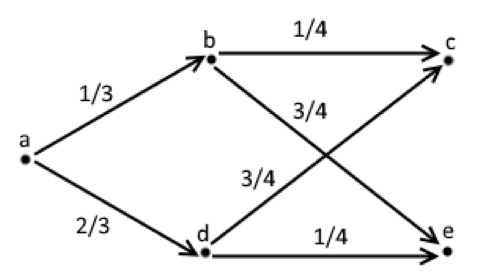
\includegraphics[width=200px]{Fig1}
\end{center}

If we have states $a, b, c$, then to find the probability of going from a to c through b $p(a, b, c)$, we have to compose them. This works by finding all the intermediate steps. $p(a, b) \times p(b, c) = p(a, b, c)$. In the example above, $p(a, b, c) = 1/12$

The same works for probability amplitudes. $\psi(a, b, c) = \psi(a, b) \times \psi(b, c)$.

\subsubsection{Composition of Different Sequences}

This is when we want to get from one state to another, but can use multiple sequences. 

$p(a, b, c) = p(a, b) \times p(b, c)$

$p(a, d, c) = p(a, d) \times p(d, c)$

$p(a, c) = p(a, b, c) + p(a, d, c) = (p(a, b) \times p(b, c)) + (p(a, d) \times p(d, c))$

Stochastic and Quantum Transition systems work in exactly the same way during composition of sequences.

However, when converting the Quantum System back into a Transition System, some odd things can happen!

$p_Q(a, c) = (p_Q(a, b) \times p_Q(b, c)) + (p_Q(a, d) \times p_Q(d, c))$

However, $p_Q(a, b) = |\psi(a, b)|^2$. (By the way, I'm going to stop writing the $\times$ explicitly...)

$p_Q(a,c) = \lvert \psi(a,b)\psi(b,c) + \psi(a,d)\psi(d, c) \rvert^2$

$p_Q(a,c) = \lvert \psi(a,b)\psi(b,c) \rvert^2 + \lvert \psi(a,d)\psi(d,c) \rvert^2 + \psi(a,b)\psi(b,c)\psi^*(a,d)\psi^*(d,c) + \psi^*(a,b)\psi^*(b,c)\psi(a,d)\psi(d,c)$

Now the above looks quite scary, but it's the simple $(ab + cd)^2$ expansion. Also, $\psi*(a,b)$ is the complex conjugate of $\psi(a,b)$.\pagebreak

\section{Linear Algebra}

\subsection{Dirac Notation}

Dirac Notation (Aka Bra-ket) notation is used for describing quantum states. $\lvert x \rangle$ is called a bra, and $\langle y \rvert$ is called a ket. Hence $\langle x \vert y \rangle$ is a bra-ket.

A bra $\langle x \rvert$ denotes a row vector $\begin{bmatrix}x_1 & ... & x_n\end{bmatrix}$.

A ket $\lvert y \rangle$ denotes a column vector $\begin{bmatrix}y_1\\...\\y_n\end{bmatrix}$. 

To save space in documents, we sometimes write a column vector as $\begin{bmatrix}x_1 & ... & x_n\end{bmatrix}^T$, where T stands for transpose. Just imagine rotating it clockwise by 90 degrees.

\subsubsection{Vector multiplication}

There's two main types of vector multiplication: inner product and outer product. 

The inner product is when you multiply a \textbf{bra} by a \textbf{ket} $\langle x \lvert y \rangle$. This returns a scalar (a number), and is calculated by multiplying together each pair of entries at each index, then add up the result.

$ \langle x \lvert y \rangle = \begin{bmatrix}x_1 & ... & x_n\end{bmatrix} . \begin{bmatrix}y_1\\...\\y_n\end{bmatrix} = x_1y_1 + x_2y_2 + ... + x_ny_n$

The outer product is when you multiply a \textbf{ket} by a \textbf{bra} $\lvert x \rangle \langle y \rvert$. This returns a matrix, and is defined as follows:

$\lvert x \rangle \langle y \rvert = \begin{bmatrix}x_1\\...\\x_n\end{bmatrix} \times \begin{bmatrix}y_1 & ... & y_n\end{bmatrix} = \begin{bmatrix} x_1y_1 & ... & x_1y_n \\ ... & & ... \\ x_ny_1 & ... & x_ny_n\end{bmatrix}$

\subsection{Complex Inner Product Space}

This is a type of set $H$ of vectors, which has an inner product defined. Here, it is important to understand what each of these are saying, rather than brute force learning them. The properties of the set are as follows:

\begin{itemize}
	\item Any two vectors in the set are \textbf{commutative under addition}: \\$\lvert x \rangle, \lvert y \rangle \in H \implies \lvert x \rangle + \lvert y \rangle = \lvert x + y \rangle = \lvert y \rangle + \lvert x \rangle \in H$.
	\item Any three vectors in the set are \textbf{associative under addition}: \\$\lvert x \rangle, \lvert y \rangle, \lvert z \rangle \in H \implies (\lvert x \rangle + \lvert y \rangle) + \lvert z \rangle = \lvert x \rangle (\lvert y \rangle + \lvert z \rangle)$
	\item The set \textbf{contains a zero element}, which does nothing when applied to a vector:\\$\underline{0} \in H$ and $\underline{0} + \lvert x \rangle = \lvert x \rangle \in H$
	\item \textbf{Closed under scalar multiplication. }Any vector can be scaled by a scalar (a number which is not a vector), and will remain in the set: \\$\lvert x \rangle \in H, \lambda \in \mathbb{C} \implies \lvert \lambda x \rangle = \lambda \lvert x \rangle \in H$
	\item \textbf{Closed under composition of scalars: }\\$\lvert x \rangle \in H , \lambda, \mu \in \mathbb{C} \implies \lvert \lambda \mu x \rangle = \lambda \lvert \mu x \rangle = \lambda \mu \lvert x \rangle \in H$
	\item \textbf{Distributive under scalar multiplication:} (for vectors)\\$\lvert x \rangle, \lvert y \rangle \in H, \lambda \in \mathbb{C} \implies \lambda(\lvert x \rangle + \lvert y \rangle) = \lambda \lvert x \rangle + \lambda \lvert y \rangle \in H$ 
	\item \textbf{Distributive under scalar multiplication:} (for scalars)\\$\lvert x \rangle, \in H, \lambda, \mu \in \mathbb{C} \implies (\lambda + \mu)\lvert x \rangle = \lambda \lvert x \rangle + \mu \lvert x \rangle \in H$ 
\end{itemize}

The inner product also has some properties:

\begin{itemize}
	\item \textbf{The inner product exists}:\\$\lvert x \rangle, \lvert y \rangle \in H \implies \langle y \vert x \rangle \in \mathbb{C}$
	\item \textbf{The inner product is equal to its complex conjugate:}\\$\langle x \vert y \rangle = \langle y \vert x \rangle^*$
	\item \textbf{The inner product is distributive:}\\$\langle z \rvert (\lvert x \rangle + \lvert y \rangle) = \langle z \vert x \rangle + \langle z \vert y \rangle$
	\item A scalar can be swapped from one side of an inner product to another, as long as you take its complex conjugate:\\$\mu \in \mathbb{C} \implies \langle y \vert \mu x \rangle = \mu \langle y \vert x \rangle = \langle \mu^*y \vert x \rangle$
	\item If we have a non-negative inner product of the same vector, if it is 0, then the vector itself must be 0\\$\langle x \vert x \rangle \geq 0$ and $\langle x \vert x \rangle = 0 \implies \lvert x \rangle = \underline{0}$
\end{itemize}

We denote the complex inner product space of column vectors as either $\mathbb{R}^n$ for vectors with only real entries, and $\mathbb{C}^n$ for vectors which can contain complex entries. The $n$ represents the number of elements in the vector, so $[1, 1+i, 1]^T \in \mathbb{C}^3$.

\subsection{Properties of Vectors}

\subsubsection{Norms}
The \textbf{norm} of a vector is a way we measure its size. We denote the norm of $\lvert x \rangle$ as $\lvert \lvert x \rvert \rvert$. The way we find this is by finding the inner product between a vector and itself, then finding the square root of that.

\begin{center}
	$\lvert \lvert x \rvert \rvert = \sqrt{\langle x \vert x \rangle}$
\end{center}

\subsubsection{Orthogonality}
Two vectors are said to be \textbf{orthogonal} if their inner product is 0. More formally, if $\langle x \vert y \rangle = 0$ then $\lvert x \rangle, \lvert y \rangle$ are orthogonal.

\begin{center}
	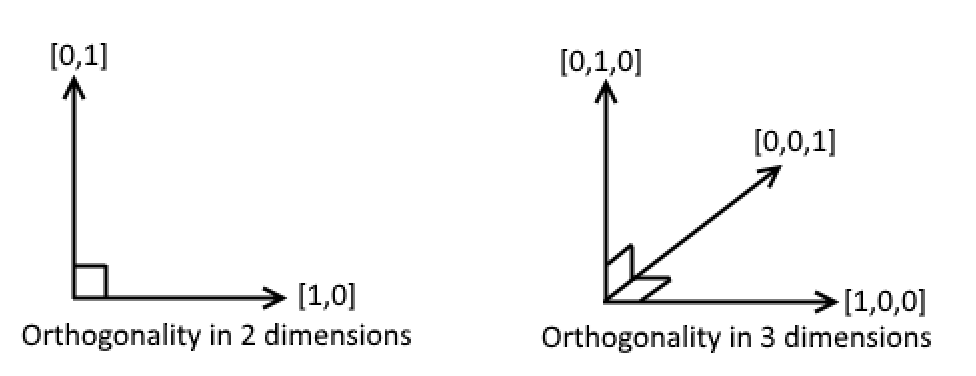
\includegraphics[width=300px]{Fig2}
\end{center}

Geometrically, if each pair of vectors are a right angle to each other, they are said to be orthogonal.

\subsubsection{Independence}

$\lvert x_0 \rangle, \lvert x_1 \rangle, \dots \lvert x_d \rangle$ are independent if they are not multiples of each other. That means we can't take some number, multiply it to a vector, and get another in our set.

$\begin{bmatrix} 1 \\ 2 \\ 3 \end{bmatrix}$ and $\begin{bmatrix} 3 \\ 6 \\ 9 \end{bmatrix}$ are not independent, because $3\begin{bmatrix} 1 \\ 2 \\ 3 \end{bmatrix} = \begin{bmatrix} 3 \\ 6 \\ 9 \end{bmatrix}$.

$\begin{bmatrix} 1 \\ 0 \\ 0 \end{bmatrix}$ and $\begin{bmatrix} 0 \\ 1 \\ 0 \end{bmatrix}$ are independent, because there is no way we can scale the first to the second. \\

If two vectors are \textbf{orthogonal}, then they are also \textbf{independent}.

Formally, $\lvert x_0 \rangle, \lvert x_1 \rangle, \dots \lvert x_d \rangle$ are independent if $\lambda_0 \lvert x_0 \rangle + \lambda_1 \lvert x_1 \rangle + \dots + \lambda_d \lvert x_d \rangle = \underline{0} \implies \lambda_0 = \lambda_1 = \dots = \lambda_d = 0$

\subsubsection{Basis}
I'll now introduce the idea of a linear combination. A linear combination is when we take multiples of different vectors, and then add them together to make a different vector. For example:

$\begin{bmatrix} 1 \\ 0 \\ 0 \end{bmatrix} + 2\begin{bmatrix} 2 \\ 0 \\ 0 \end{bmatrix} - 5\begin{bmatrix} 0 \\ 0 \\ 2 \end{bmatrix} = \begin{bmatrix} 5 \\ 0 \\ -10 \end{bmatrix}$.

Now, if we have a set of vectors which can be combined in such a way which can create any vector in the given complex inner product space, then we say that this set \textbf{spans} the space. The example above cannot produce $[0 , 1, 0]^T$, hence does not span the set of all 3 dimensional vectors.

Now, if we have a set of vectors which spans the entire space, \textbf{and} each of them are independent, then we say this set is a \textbf{basis}. 

1D Basis: $\{\begin{bmatrix} 1 \end{bmatrix}\}$ 

2D Basis: $\{\begin{bmatrix} 1 \\ 2 \end{bmatrix}, \begin{bmatrix} 0 \\ 1 \end{bmatrix}\}$ or $\{\begin{bmatrix} 1 \\ 0 \end{bmatrix}, \begin{bmatrix} 0 \\ 2 \end{bmatrix}\}$ (there are other examples...)

3D Basis: $\{\begin{bmatrix} 1 \\ 0 \\ 0\end{bmatrix}, \begin{bmatrix} 0 \\ 1 \\ 0\end{bmatrix}, \begin{bmatrix} 0 \\ 0 \\ 1\end{bmatrix}\}$ (and plenty of others...)

Hence, we can say the basis \textbf{spans} the whole space. 

The \textbf{dimension} of a space is the number of vectors in the basis. This is obvious from the example above, and fits our intuitive understanding of dimensions. This is denoted $dim(H)$

A basis is \textbf{orthogonal} if each of its vectors are orthogonal to one another. The second 2D basis above is orthogonal.

A basis is \textbf{orthonormal} if each vector has a norm of 1, and are orthogonal. The 1D basis and 3D basis above are orthonormal.

\subsection{Some Identities}

This will be filled in when I have the patience... :) \pagebreak

\section{Linear Operators}
An \textbf{operator} in Quantum Physics is something which maps an element from one complex (inner product) space (say $H_1$) to another complex space (say $H_2$). It can be thought of being like a function. $A(\lvert x \rangle) = A \lvert x \rangle$, where $\lvert x \rangle$ is the input, and $A\lvert x \rangle$ is the output.

An example of an operator could be A = \textit{multiply by 2}. $A(2) = 4$.

An operator is a \textbf{linear operator} if we can also take two scalars $\lambda, \mu$, and two vectors from $H_1$, $\lvert x \rangle, \lvert y \rangle$, so that when we apply the operator to a linear combination, it is still a linear combination. 

$A(\lambda \lvert x \rangle + \mu \lvert y \rangle) = \lambda A \lvert x \rangle + \mu A \lvert y \rangle$.

Usually, a linear operator maps from a complex space back into itself, such that $H_1 = H_2$.

If we have $H = \mathbb{C}^n, n \geq 2$, then the operators are $n \times n$ matrices, which we denote $\mathbb{C}^{n \times n}$.

\subsection{Examples of linear operators}

\subsubsection{Null Operator}

For all $\lvert x \rangle$, $\textbf{0} \lvert x \rangle = \underline{0}$
.This simply maps every vector to the zero vector.

$\begin{bmatrix} 0 & 0 \\ 0 & 0 \end{bmatrix} \times \begin{bmatrix} 5 \\ 8 \end{bmatrix} = \begin{bmatrix} 0 \\ 0 \end{bmatrix}$

\subsubsection{Identity Operator}

For all $\lvert x \rangle, \textbf{I}\lvert x \rangle = \lvert x \rangle$. In other words, the identity operator doesn't change the given vector, i.e it maps it back to itself.

$\begin{bmatrix} 1 & 0 \\ 0 & 1 \end{bmatrix} \times \begin{bmatrix} 2 \\ 5 \end{bmatrix} = \begin{bmatrix} 2 \\ 5 \end{bmatrix}$

\subsubsection{Wave Function Operators}

\textbf{Position Operator}\\
On $L_2(\mathbb{R})$ the operator $x$ which sends $f(x) \rightarrow x.f(x)$.\\
Here, $L_2$ means 2-dimensional vectors of real numbers, and the operator multiplies the input by x.

\textbf{Momentum Operator}\\
On $L_2(\mathbb{R})$, the operator $p$ which sends $f(x) \rightarrow -i\frac{df}{dx}$. This says "differentiate by $x$ and multiply by $-i$'.

These two operators when used together are used to describe the functions representing a one dimensional wave.

\subsubsection{Pauli Spin Matrices}
Later on in the course, we begin to consider the spin of electrons. These matrices presented are very useful for these calculations, hence it is very useful just to "brute memorise" these matrices.

\begin{center}
	$\sigma_x = \begin{bmatrix} 0 & 1 \\ 1 & 0 \end{bmatrix}, \sigma_y = \begin{bmatrix} 0 & -i \\ i & 0 \end{bmatrix}, \sigma_z = \begin{bmatrix} 1 & 0 \\ 0 & -1 \end{bmatrix}, \textbf{I} = \begin{bmatrix} 1 & 0 \\ 0 & 1 \end{bmatrix}$
\end{center}

They also adhere to the following properties:

\begin{center}
	$\sigma_x\sigma_y = i\sigma_z = -\sigma_y\sigma_x$\\
$\sigma_y\sigma_z = i\sigma_x = -\sigma_z\sigma_y$\\
$\sigma_x\sigma_z = i\sigma_y = -\sigma_z\sigma_x$\\
$\sigma_x^2 = \sigma_y^2 = \sigma_z^2 = \textbf{I}$\\
$\sigma_x^\dag = \sigma_x; \sigma_y^\dag = \sigma_y; \sigma_z^\dag = \sigma_z$
\end{center}

\subsection{Composition of Operators}


\subsection{Power Series}


\subsection{Matrix Elements}


\subsection{Special Operators}


\subsection{Diagonalisation}


\subsection{Change of Basis}

\pagebreak

\section{Constructions in Spaces}

\section{Fundamentals Quantum Theory}

\section{Quantum Entanglement}

\section{Fundamentals of Quantum Computing}

\end{document}
